\chapter{Nuclear Shape Deformations}

Rick Casten has given several lectures about nuclear shape deformations and other such things. A lot of this will probably just be restating things he has said in my own words.

First of all, one important tool that you should understand in order to talk about nuclear shape deformations is a Nilsson diagram. First of all, you've seen level diagrams in atomic and nuclear spectroscopy. Figure \ref{fig:NuclearShells}, for instance, is a familiar illustration of low-lying energy levels for a harmonic oscillator potential, both before and after adding a spin-orbit interaction term which leads to the well-known nuclear "magic numbers."

\begin{wrapfigure}{R}{0.5\textwidth}
%\centering
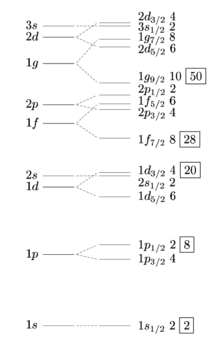
\includegraphics[width=0.45\textwidth]{TeX_files/NuclearShells}
\caption[Nuclear Shell Model level diagram]{From Wikipedia: "Low-lying energy levels in a single-particle shell model with an oscillator potential (with a small negative l2 term) without spin-orbit (left) and with spin-orbit (right) interaction. The number to the right of a level indicates its degeneracy, (2j+1). The boxed integers indicate the magic numbers."}
\label{fig:NuclearShells}
\end{wrapfigure}

Now imagine you stretch out the nucleus somehow. That'll certainly change the spacing and position of the energy levels, because some electron orbitals have a sort of intrinsic shape characteristic that might be better- or worse-suited for the new elongation.

Finally, imagine that you do the stretching \textit{continuously}. That is what is done in a Nilsson diagram. For example, in figure \ref{fig:NilssonDiagram}, the system is elongated from a spherical ground state, and the changing energy levels are the curves, which frequently end up crossing one another. An important thing to notice is that, for different deformations you might have different shell gaps, and as well you might find that different orbitals are more favorable at different deformations.

\begin{figure}
\centering
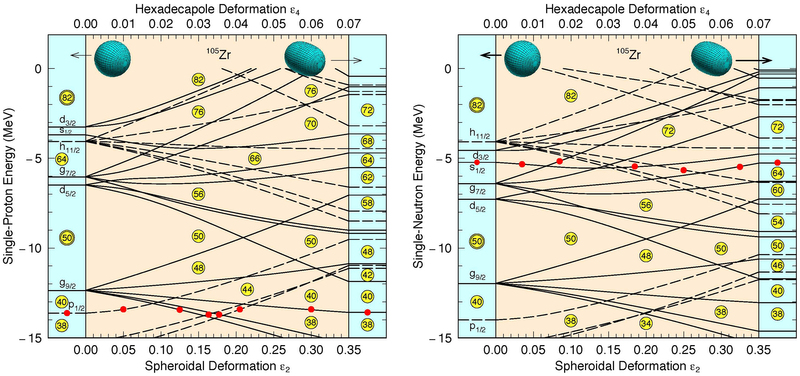
\includegraphics[width=0.7\linewidth]{TeX_files/NilssonDiagram}
\caption[Nilsson Diagram for Zr-105]{Nilsson Diagram for Zr-105, plotted against elongation parameter $\epsilon_2$}
\label{fig:NilssonDiagram}
\end{figure}

Anyway, that's all helpful \textit{once you know} the deformation. And there's a lot of useful and interesting things you can say and predict using a Nilsson diagram - heck, if you know the shape you can [qualitatively] even \textit{draw} a Nilsson diagram, just by thinking about the physical system and how the orbitals are probably behaving.  BUT if you want to understand why a nucleus deforms in the first place, that's a whole other story.

\section{What causes nuclear ground state deformations?}

As with most peculiarities of nuclear structure, the source of nuclear deformation is primarily an artifact of shell structure. In particular, when there is a large shell gap, the nucleus will get sort of "locked" into a particular stable configuration, and if that happens to be a deformed configuration because of the orbital characteristics of the outermost nucleons (because that's the only thing that could matter, right?), then so be it.

A question that I have is how is there ground state deformation in even-even nuclei? Because even-even nuclei all have, without exception, spin-parity $0^+$, and yet $^{152}Dy$ (for example) is highly-deformed. Am I misunderstanding the implications of such a spin-parity assignment? Or am I misunderstanding what is meant by "ground state deformed"?

I don't think this is a real answer, but one way to identify even-even deformed nuclei is to look for nuclei with a large $\frac{E(4^+)}{E(2^+)}$ ratio (or a related method is to look for those with a relatively-small $E(2^+)$).

\section{Phenomenology of Nilsson Diagrams}

[Basically here is where you were thinking about Casten's slides. He goes through and talks about whether a level's energy will go up or down, and how it will curve, just by thinking about the orbital motion of single particles around different axes of the deformed system.]

\section{What causes nuclear ground state deformations? Part 2}
\subsection{What causes fission?}

I think there's a couple of effects at play that lead to fission. First of all, what gets the nucleus moving in the first place, and second, what \textit{keeps} it moving?

To answer the first question, imagine you were to buy a bunch of nucleons at the store and then put them in a box together. Just dump them in with some arbitrary configuration. They'll start to attract and repel one another and there will be kind of a chaotic mess of particle motions to keep track of. TDHF will kind of give you a sense of what's going on in sort of an average sense.

Eventually, the system might settle into a set of sort of normal modes. There will probably be several overlapping normal modes happening at once, so the motion will still look pretty chaotic, but in some average sense you might get something that starts to move with some pseudo-regularity. And with time (I suppose regardless of whether the system motion os regular or not), the system might (for example) elongate, and in fact it might elongate enough for there to be a level crossing in the Nilsson diagram.

When this happens, the system has some deciding to do. It might continue on its current trajectory, or it might jump onto another trajectory (that is, there might be a nucleonic transition from one energy level to another). I suppose it is pretty difficult in practice for a nucleon to make these transitions, because you have all kind of things like conservation of angular momentum and Pauli's principle and such to consider. BUT if you transition a pair of nucleons instead of just one, you can skirt around a lot of these issues, and so I think that's what frequently tends to happen. That is why pairing correlations are sometimes called the "lubricant" of nuclear fission \cite{Bulgac2016}.

To go further brings you into the world of diabatic vs adiabatic level crossings. Witek talks about this in \cite{Nazarewicz1993} (and that's what I'm trying to read through and understand right now). First, some terminology: The words ``diabatic" and ``adiabatic" come from Greek: ``a"= ``not", ``dia"=``through", ``batok"=``passable." So at a diabatic level crossing, the levels just pass right through one another without interacting or acknowledging one another. At an adiabatic level crossing, there might be some kind of level mixing as a result of residual interactions (basically, your single-particle picture wasn't good enough, I suppose). This is the point being illustrated in figure 1 of that reference: In the diabatic picture, you have two independent harmonic oscillators that happen to occupy the same space, whereas in the adiabatic picture, you have just a couple of messy, non-symmetric potential wells.

\section{Describing Scission}

(This is probably way out of place, but whatever...) Intuitively, you might think that the driving factor which determines fragment ID distributions would be shell structure of the fragments. And if I'm reading this right \cite[2nd paragraph + references]{Mcdonnell2014}, you'd be partly right: the \textit{real} driving factor is shell structure of the \textit{prefragments}, and an important factor in understanding this is that the prefragments are typically highly-deformed, which means that their shell structure is probably totally different than it would be for those same fragments in their ground state.